\byline{{\textbf{\Large\sffamily Bonsai Events:}}\\
        {\textbf{\large\sffamily The 14th Heathrow Bonsai Show}}}{Stefano Bragaglia}
\label{2025-10-show}
\noindent
On Sunday, 5th October 2025, the UK bonsai world gathered once again for the much\--anticipated \href{https://heathrowbonsai.weebly.com}{14th Heathrow Bonsai Show}, held at the spacious and bright \textit{Bracknell Leisure Centre}, Berkshire.
After a few days of worry about the first autumn storm of the season, it was a relief to wake up to calm skies and golden sunshine.
I travelled over where I have met with a few fellow enthusiasts from our club, all sharing that eternal question: did we have enough cash for the traders?

The Heathrow Show has become one of the fixtures of the UK bonsai calendar: a celebration of club enthusiasm rather than high\--end competition, where trees in advanced stage of development from all over the country can be admired and discussed.
This year's edition featured an impressive \textbf{38 club displays}, each a labour of love representing the creative diversity of the British bonsai community.
From the refined classical arrangements of the \href{https://www.southendbonsai.com}{Southend Bonsai Society} to the bold, contemporary styling of the \href{https://exeterbonsaisociety.com}{Exeter Bonsai Society}, the show floor buzzed with energy and conversation.

Walking in, the first impression was one of abundance.
Rows of carefully lit tables stretched across the hall, each adorned with trees of every size, from stately pines to delicately trained shohin.
The \href{https://ukminibonsaigroup.weebly.com}{UK Mini Bonsai Group} drew plenty of smiles with their collection of perfectly formed miniatures --- always a crowd favourite --- while newer societies such as \href{http://www.celticknotbonsai.co.uk}{Celtic Knot Bonsai} and \textit{Creative Companions} brought a refreshing sense of experimentation to their compositions.

The spirit of collaboration was palpable.
Clubs travelled from far and wide: from Cornwall and Wales to the East of England, with groups including \textit{Bedfordshire}, \textit{Salisbury}, \textit{North London}, \textit{Mid\--Herts}, \textit{Sussex}, \textit{Swindon}, and many more.
It was, quite literally, a meeting of the nation's bonsai minds.
A few visitors commented that each year the displays grow stronger and more cohesive --- proof that the Heathrow formula continues to nurture talent and encourage participation from all corners of the hobby.

As in previous years, the show featured the popular ``\textit{My Favourite Top Three Displays}'' competition, voted for by the visiting public.
There had been some debate within the UKBA steering group about whether to retire the contest, in order to avoid the occasional controversy that accompanies judging.
However, it was ultimately decided that it added to the sense of engagement and fun for visitors --- and, as it turned out, the crowds agreed.
Over 600 ballots were cast, and the results reflected both consistency and surprise in equal measure.

\textbf{1st place} went to the superbly balanced display from \textbf{Southend Bonsai Society}, whose naturalistic pines and harmonious accents captured the imagination of all who saw them.
\textbf{2nd place} went to \textbf{Sutton Bonsai Society}, whose group planting of evergreens evoked a peaceful woodland glade.
\textbf{3rd place} went to \textbf{Exeter Bonsai Society}, showcasing a beautifully presented mixed species display with a striking scroll depicting mist rising through pines.
The top twenty club displays were also published for the first time this year, a thoughtful gesture that acknowledged the breadth of quality across the show.
The \textit{South Wales Bonsai Collective}, \textit{Somerset}, \textit{Cardiff}, and \textit{Swindon} clubs all earned strong positions, while groups such as ours, \textit{Twickenham Bonsai}, and \textit{Middlesex Bonsai Society} were delighted to see their names among the voted favourites.

The traders' area was as vibrant as ever --- a veritable treasure trove for enthusiasts and newcomers alike.
Familiar faces such as \href{https://www.instagram.com/walsallstudioceramics/}{Walsall Studio Ceramics}, \href{https://deiceramics.com}{Dei Ceramics}, and \href{https://grainoftime.co.uk}{Grain of Time} were joined by a host of others, including \href{https://www.beechfieldbonsai.co.uk/}{Beechfield Bonsai}, \href{https://www.bonsai.co.uk}{Greenwood Bonsai}, \href{https://www.davidcheshirenurseries.co.uk}{David Cheshire Bonsai}, \href{https://www.facebook.com/p/Spectre-ceramics-100065407593513/}{Spectre Ceramics}, \href{https://www.instagram.com/shohinuk/}{Shohin Bonsai} and the ever\--popular \href{https://bonsai4me.com}{Bonsai4Me}.
Every corner of the hall seemed to offer temptation --- a pot that might just fit that awkward maple, a piece of material too beautiful to leave behind, or a set of tools that gleamed just a little too invitingly.

Several traders remarked how brisk business was throughout the day, helped by the strong attendance.
With nearly \textbf{a thousand people} passing through the venue --- including exhibitors, vendors and visitors --- the atmosphere was lively yet unhurried.
Conversations flowed easily; old friends caught up, and new ones were made over shared admiration of a particularly fine beech or juniper.
It was everything a bonsai event should be: educational, inspiring, and sociable in equal measure.

One could not fail to notice the seamless organisation behind it all.
The Heathrow team has become a model of efficiency, with setup and breakdown executed in record time.
As one volunteer joked, ``By the time you've had your first coffee, the whole show's up!''
This professionalism allows the event to retain its friendly charm while managing the logistics of such a large gathering --- no small feat given the number of participants involved.

There were, of course, many small moments that summed up the day: a child marvelling at a tiny oak, a quiet conversation between two seasoned growers about soil composition, a burst of laughter from a group of exhibitors after a long day's packing.
These are the details that make the Heathrow Bonsai Show more than just an exhibition; it is, at heart, a community celebration of shared passion and patience.

As the sun dipped lower and the last trees were carefully packed away, there was a genuine sense of satisfaction in the air.
The Heathrow Show continues to prove that bonsai in the UK is alive, growing, and thriving across all levels.
Whether you came to display, to buy, or simply to be inspired, it was a day that reminded us why we gather each autumn: to celebrate the art, the craft, and the friendship that bonsai brings.

A heartfelt thank you goes to the organisers, the many participating clubs, and everyone who helped make this year's event a success.
Here's to another year of growth --- both for our trees and our community.
\closearticle

\end{multicols}

\begin{center}
    \begin{minipage}[b]{.4\textwidth}
        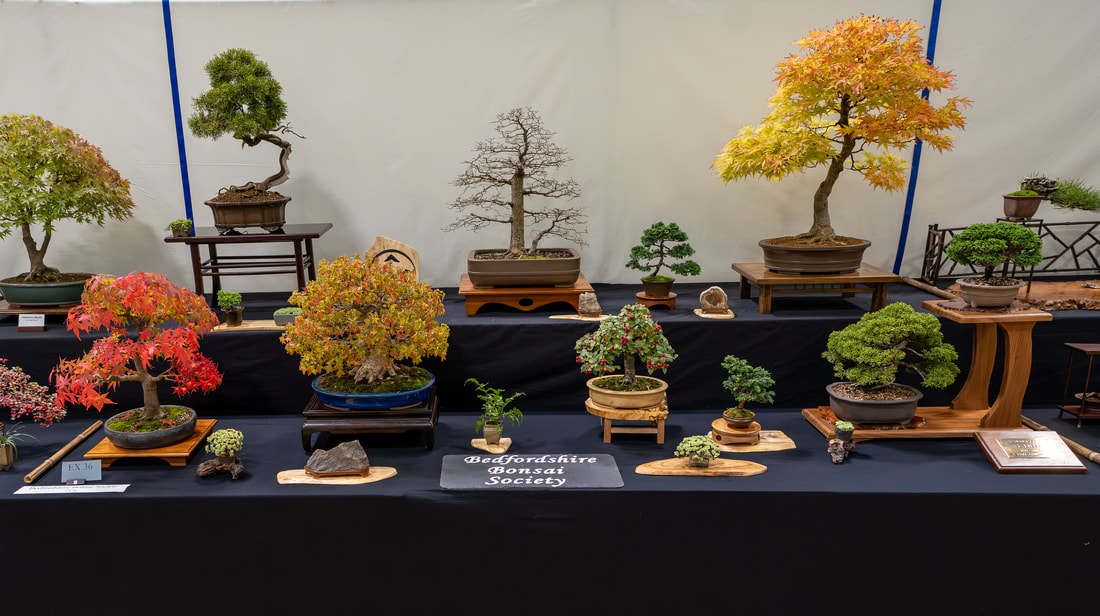
\includegraphics[angle=0,origin=c,width=1.0\textwidth]{2025_10/res/heathrow_01_bedfordshire_bonsai_society}
        \centerline{\emph{Bedfordshire Bonsai Society}}
    \end{minipage}\quad
    \begin{minipage}[b]{.4\textwidth}
        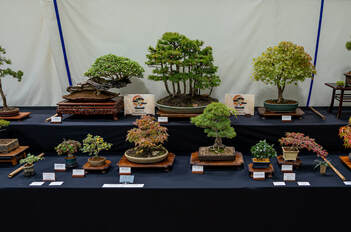
\includegraphics[angle=0,origin=c,width=1.0\textwidth]{2025_10/res/heathrow_02_berkshire_bonsai_society}
        \centerline{\emph{Berkshire Bonsai Society}}
    \end{minipage}
    \medskip

    \begin{minipage}[b]{.4\textwidth}
        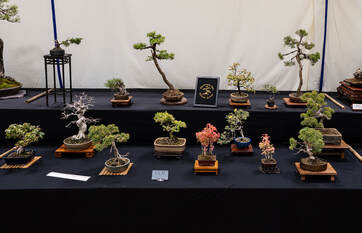
\includegraphics[angle=0,origin=c,width=1.0\textwidth]{2025_10/res/heathrow_03_blackmore_vale_bonsai_society}
        \centerline{\emph{Blackmore Vale Bonsai Society}}
    \end{minipage}\quad
    \begin{minipage}[b]{.4\textwidth}
        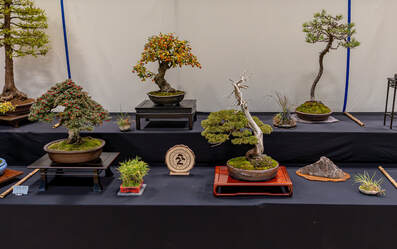
\includegraphics[angle=0,origin=c,width=1.0\textwidth]{2025_10/res/heathrow_04_bristol_bonsai_society}
        \centerline{\emph{Bristol Bonsai Society}}
    \end{minipage}
    \medskip

    \begin{minipage}[b]{.4\textwidth}
        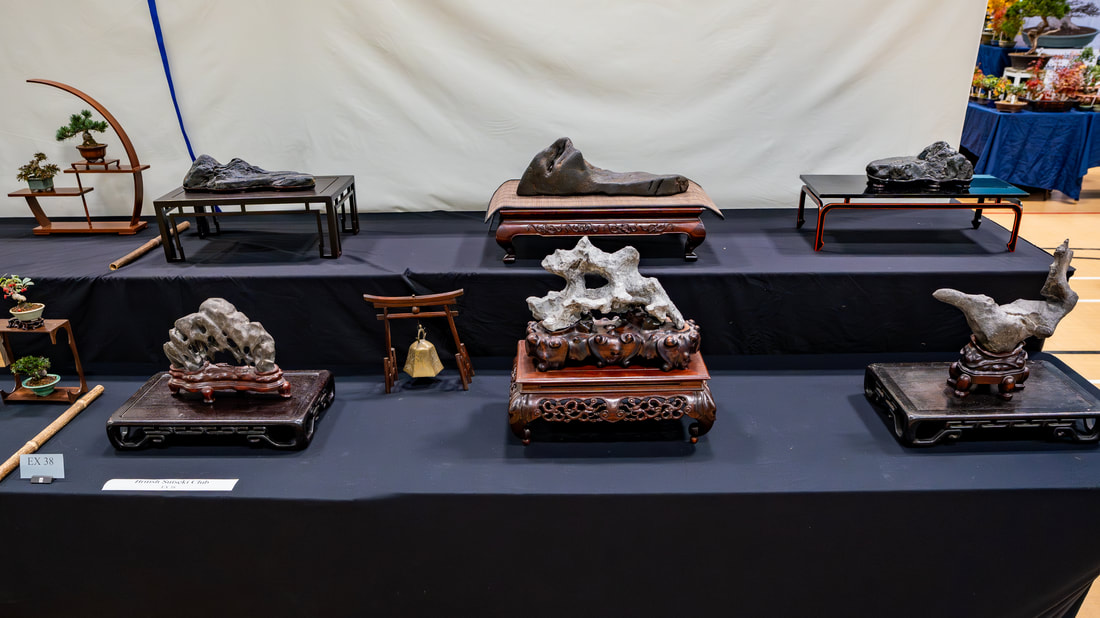
\includegraphics[angle=0,origin=c,width=1.0\textwidth]{2025_10/res/heathrow_05_british_suiseki_club}
        \centerline{\emph{British Suiseki Club}}
    \end{minipage}\quad
    \begin{minipage}[b]{.4\textwidth}
        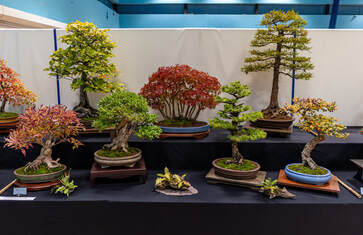
\includegraphics[angle=0,origin=c,width=1.0\textwidth]{2025_10/res/heathrow_06_cardiff_bonsai_society}
        \centerline{\emph{Cardiff Bonsai Society}}
    \end{minipage}
    \medskip

    \begin{minipage}[b]{.4\textwidth}
        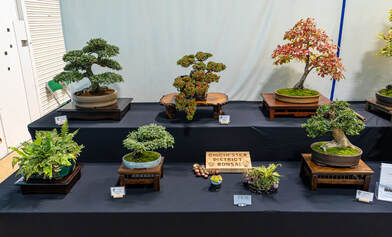
\includegraphics[angle=0,origin=c,width=1.0\textwidth]{2025_10/res/heathrow_07_chichester_bonsai_society}
        \centerline{\emph{Chichester Bonsai Society}}
    \end{minipage}\quad
    \begin{minipage}[b]{.4\textwidth}
        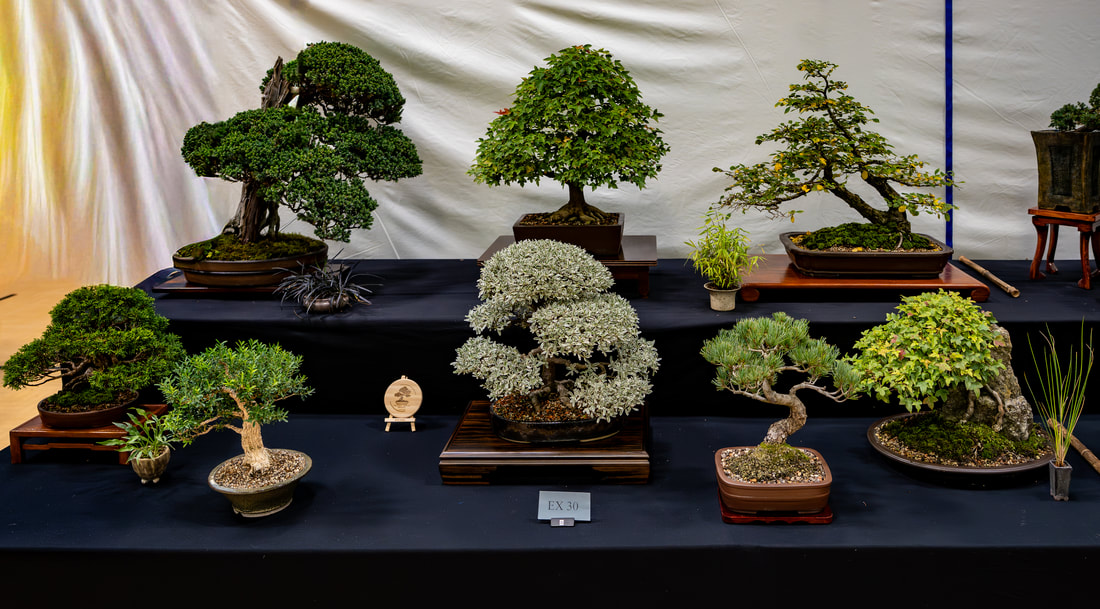
\includegraphics[angle=0,origin=c,width=1.0\textwidth]{2025_10/res/heathrow_08_chiltern_bonsai_society}
        \centerline{\emph{Chiltern Bonsai Society}}
    \end{minipage}
\end{center}
\clearpage

\begin{center}
    \begin{minipage}[b]{.4\textwidth}
        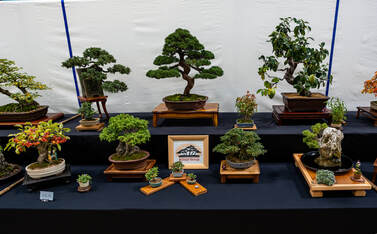
\includegraphics[angle=0,origin=c,width=1.0\textwidth]{2025_10/res/heathrow_09_crawley_bonsai_society}
        \centerline{\emph{Crawley Bonsai Society}}
    \end{minipage}\quad
    \begin{minipage}[b]{.4\textwidth}
        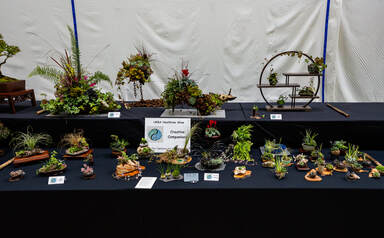
\includegraphics[angle=0,origin=c,width=1.0\textwidth]{2025_10/res/heathrow_10_creative_companions}
        \centerline{\emph{Creative Companions}}
    \end{minipage}
    \medskip

    \begin{minipage}[b]{.4\textwidth}
        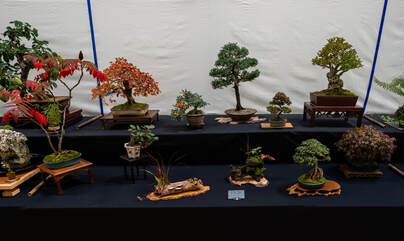
\includegraphics[angle=0,origin=c,width=1.0\textwidth]{2025_10/res/heathrow_11_dragon_bonsai_society}
        \centerline{\emph{Dragon Bonsai Society}}
    \end{minipage}\quad
    \begin{minipage}[b]{.4\textwidth}
        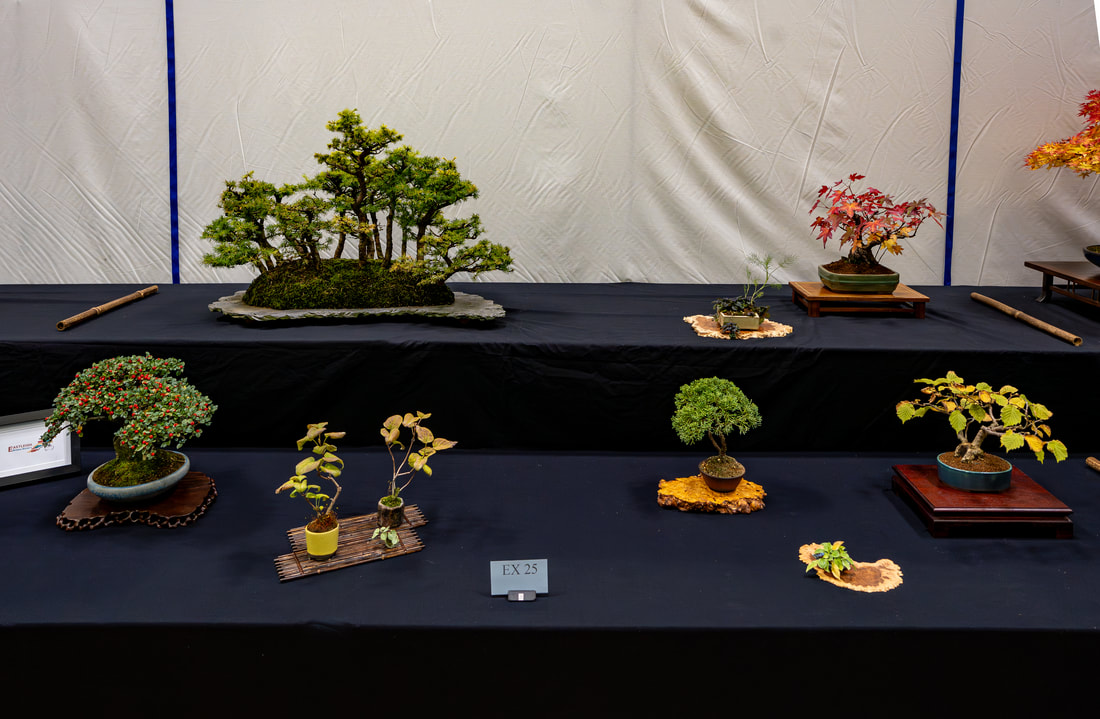
\includegraphics[angle=0,origin=c,width=1.0\textwidth]{2025_10/res/heathrow_12_eastleigh_bonsai_society}
        \centerline{\emph{Eastleigh Bonsai Society}}
    \end{minipage}
    \medskip

    \begin{minipage}[b]{.4\textwidth}
        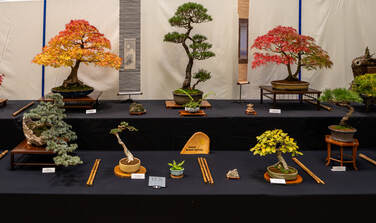
\includegraphics[angle=0,origin=c,width=1.0\textwidth]{2025_10/res/heathrow_13_exeter_bonsai_society}
        \centerline{\emph{Exeter Bonsai Society}}
    \end{minipage}\quad
    \begin{minipage}[b]{.4\textwidth}
        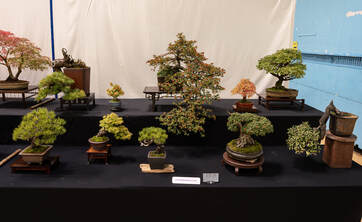
\includegraphics[angle=0,origin=c,width=1.0\textwidth]{2025_10/res/heathrow_14_glynderi_bonsai_society}
        \centerline{\emph{Glynderi Bonsai Society}}
    \end{minipage}
    \medskip

    \begin{minipage}[b]{.4\textwidth}
        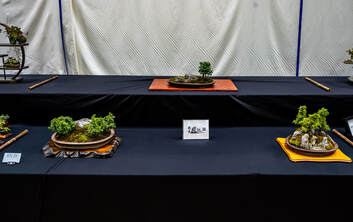
\includegraphics[angle=0,origin=c,width=1.0\textwidth]{2025_10/res/heathrow_15_international_saikei_association}
        \centerline{\emph{International Saikei Association}}
    \end{minipage}\quad
    \begin{minipage}[b]{.4\textwidth}
        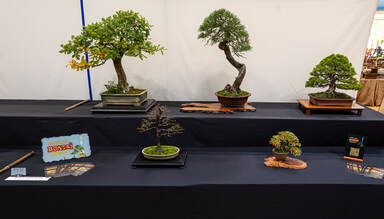
\includegraphics[angle=0,origin=c,width=1.0\textwidth]{2025_10/res/heathrow_16_ipswich_bonsai_society}
        \centerline{\emph{Ipswich Bonsai Society}}
    \end{minipage}
\end{center}
\clearpage

\begin{center}
    \begin{minipage}[b]{.4\textwidth}
        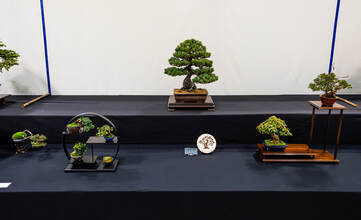
\includegraphics[angle=0,origin=c,width=1.0\textwidth]{2025_10/res/heathrow_17_liver_bonsai_group}
        \centerline{\emph{Liver Bonsai Group}}
    \end{minipage}\quad
    \begin{minipage}[b]{.4\textwidth}
        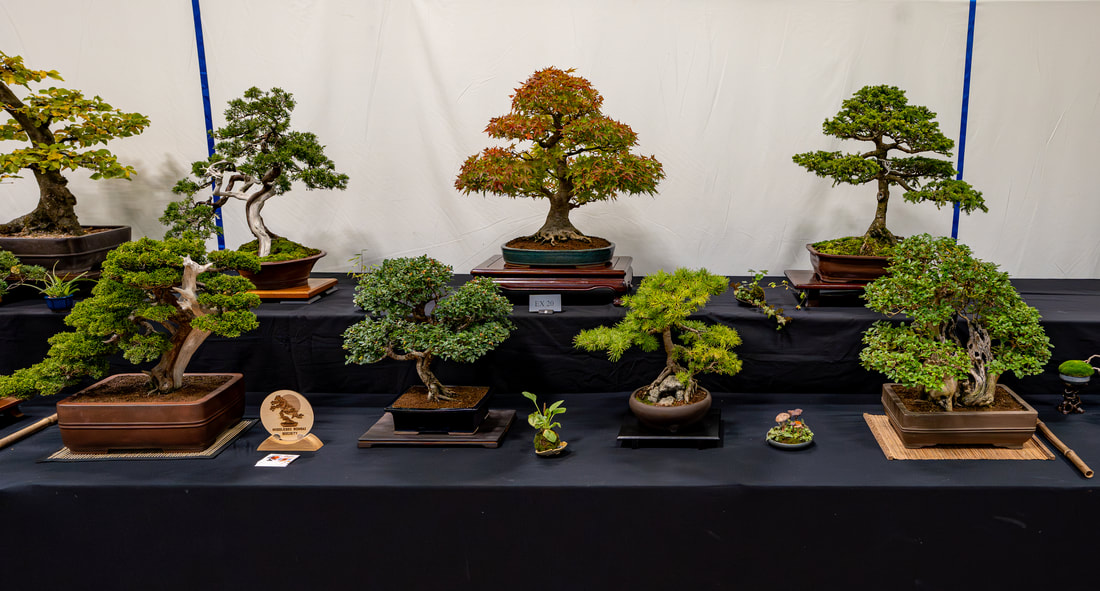
\includegraphics[angle=0,origin=c,width=1.0\textwidth]{2025_10/res/heathrow_18_middlesex_bonsai_society}
        \centerline{\emph{Middlesex Bonsai Society}}
    \end{minipage}
    \medskip

    \begin{minipage}[b]{.4\textwidth}
        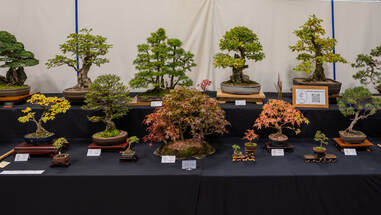
\includegraphics[angle=0,origin=c,width=1.0\textwidth]{2025_10/res/heathrow_19_mid_herts_bonsai_society}
        \centerline{\emph{Mid\--Herts Bonsai Society}}
    \end{minipage}\quad
    \begin{minipage}[b]{.4\textwidth}
        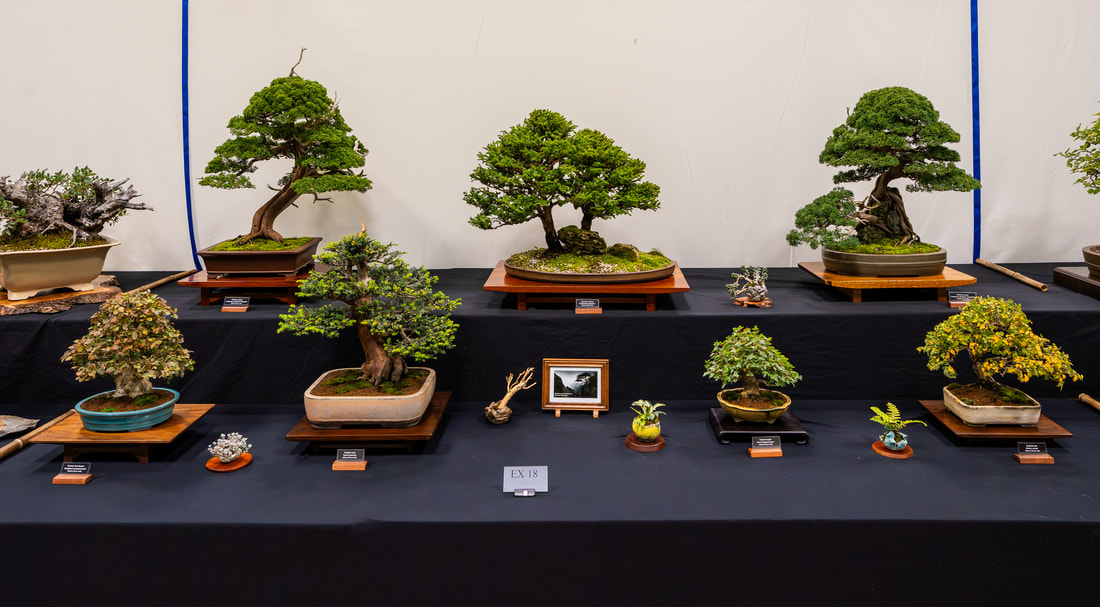
\includegraphics[angle=0,origin=c,width=1.0\textwidth]{2025_10/res/heathrow_20_newbury_bonsai_society}
        \centerline{\emph{Newbury Bonsai Society}}
    \end{minipage}
    \medskip

    \begin{minipage}[b]{.4\textwidth}
        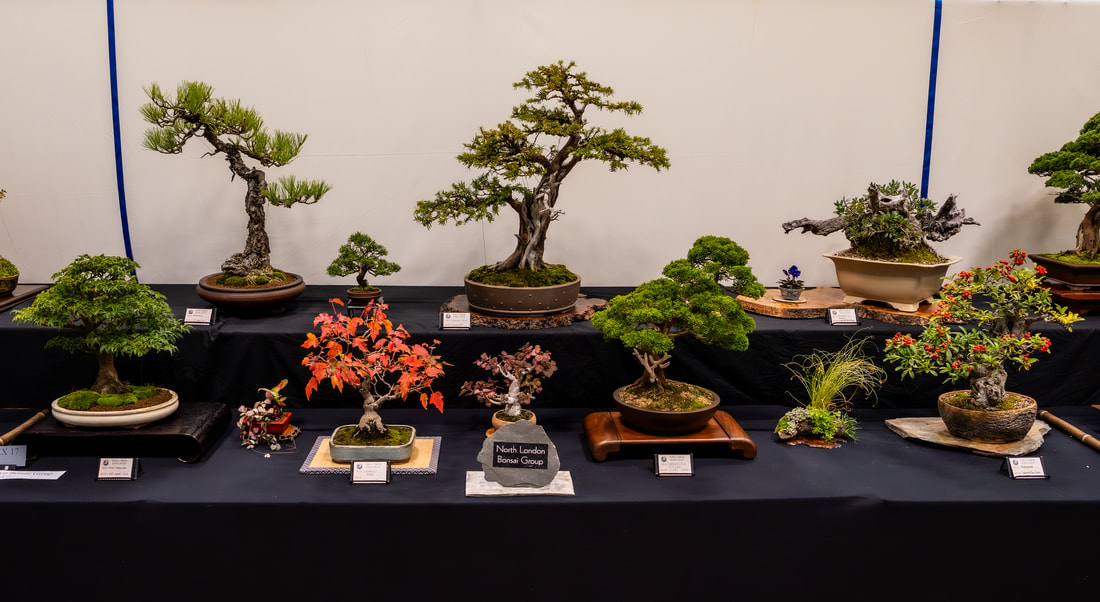
\includegraphics[angle=0,origin=c,width=1.0\textwidth]{2025_10/res/heathrow_21_north_london_bonsai_group}
        \centerline{\emph{North London Bonsai Society}}
    \end{minipage}\quad
    \begin{minipage}[b]{.4\textwidth}
        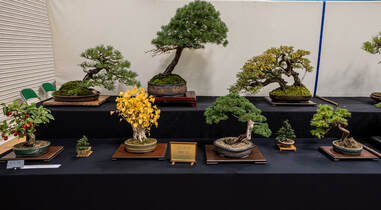
\includegraphics[angle=0,origin=c,width=1.0\textwidth]{2025_10/res/heathrow_22_salisbury_bonsai_society}
        \centerline{\emph{Salisbury Bonsai Society}}
    \end{minipage}
    \medskip

    \begin{minipage}[b]{.4\textwidth}
        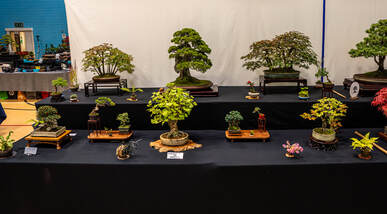
\includegraphics[angle=0,origin=c,width=1.0\textwidth]{2025_10/res/heathrow_23_solent_bonsai_society}
        \centerline{\emph{Solent Bonsai Society}}
    \end{minipage}\quad
    \begin{minipage}[b]{.4\textwidth}
        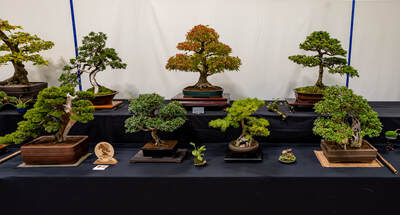
\includegraphics[angle=0,origin=c,width=1.0\textwidth]{2025_10/res/heathrow_24_somerset_bonsai_society}
        \centerline{\emph{Somerset Bonsai Society}}
    \end{minipage}
    \medskip

    \begin{minipage}[b]{.4\textwidth}
        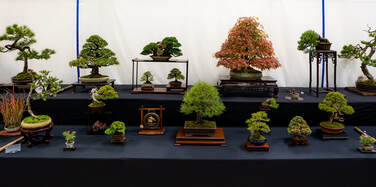
\includegraphics[angle=0,origin=c,width=1.0\textwidth]{2025_10/res/heathrow_25_south_east_bonsi_club}
        \centerline{\emph{South East Bonsai Club}}
    \end{minipage}\quad
    \begin{minipage}[b]{.4\textwidth}
        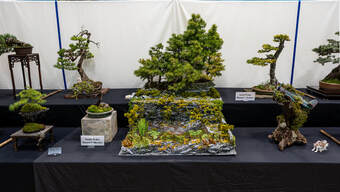
\includegraphics[angle=0,origin=c,width=1.0\textwidth]{2025_10/res/heathrow_26_south_wales_bonsai_collective}
        \centerline{\emph{South Wales Bonsai Collective}}
    \end{minipage}
\end{center}
\clearpage

\begin{center}
    \begin{minipage}[b]{.4\textwidth}
        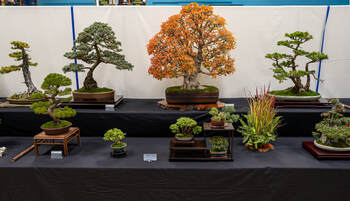
\includegraphics[angle=0,origin=c,width=1.0\textwidth]{2025_10/res/heathrow_27_southend_bonsai_society}
        \centerline{\emph{Southend Bonsai Society}}
    \end{minipage}\quad
    \begin{minipage}[b]{.4\textwidth}
        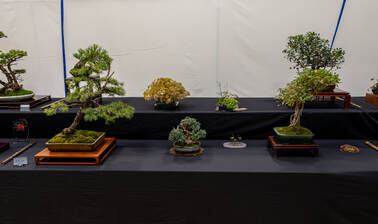
\includegraphics[angle=0,origin=c,width=1.0\textwidth]{2025_10/res/heathrow_28_splinter_bonsai_group}
        \centerline{\emph{Splinter Bonsai Group}}
    \end{minipage}
    \medskip

    \begin{minipage}[b]{.4\textwidth}
        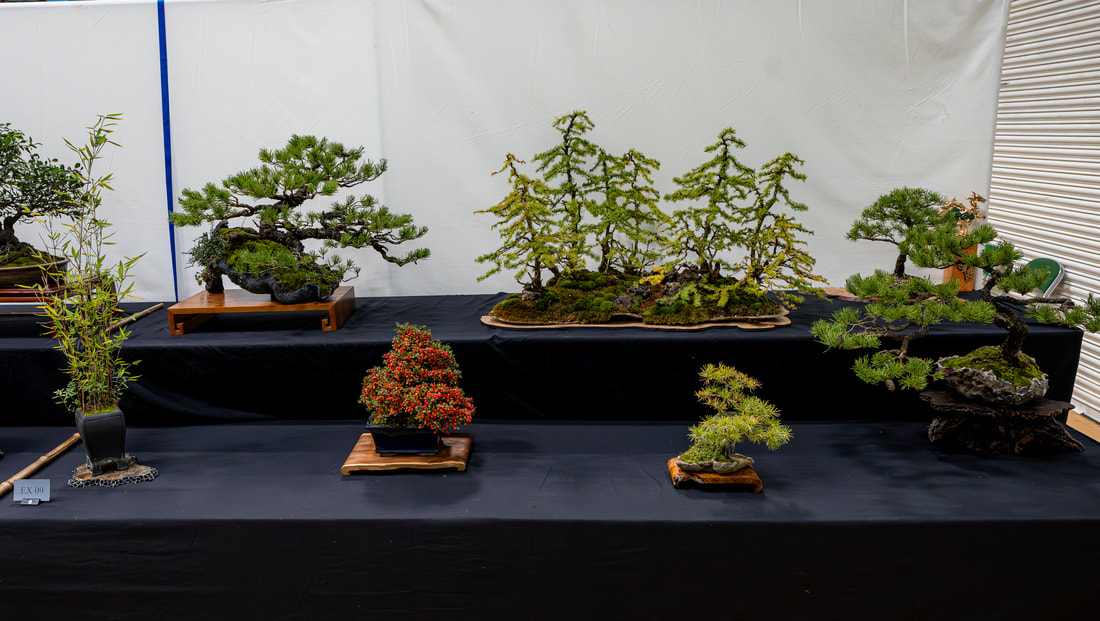
\includegraphics[angle=0,origin=c,width=1.0\textwidth]{2025_10/res/heathrow_29_staverton_bonsai_group}
        \centerline{\emph{Staverton Bonsai Group}}
    \end{minipage}\quad
    \begin{minipage}[b]{.4\textwidth}
        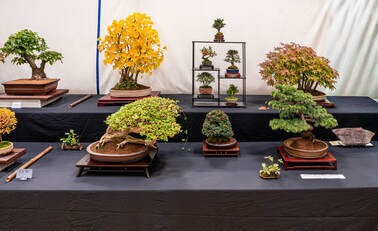
\includegraphics[angle=0,origin=c,width=1.0\textwidth]{2025_10/res/heathrow_30_surrey_heath_bonsai_society}
        \centerline{\emph{Surrey Heath Bonsai Society}}
    \end{minipage}
    \medskip

    \begin{minipage}[b]{.4\textwidth}
        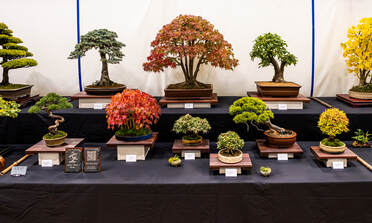
\includegraphics[angle=0,origin=c,width=1.0\textwidth]{2025_10/res/heathrow_31_sussex_bonsai_group}
        \centerline{\emph{Sussex Bonsai Group}}
    \end{minipage}\quad
    \begin{minipage}[b]{.4\textwidth}
        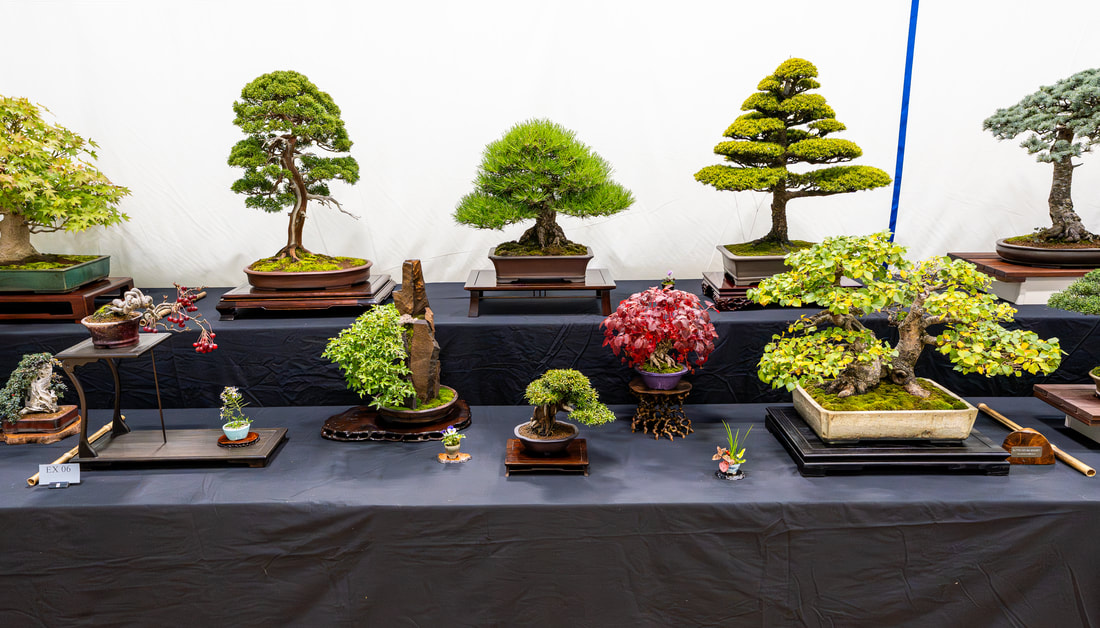
\includegraphics[angle=0,origin=c,width=1.0\textwidth]{2025_10/res/heathrow_32_sutton_bonsai_society}
        \centerline{\emph{Sutton Bonsai Society}}
    \end{minipage}
    \medskip

    \begin{minipage}[b]{.4\textwidth}
        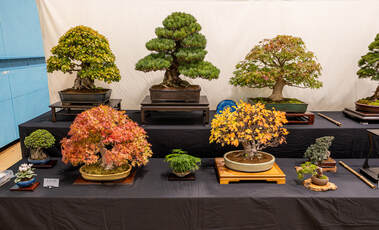
\includegraphics[angle=0,origin=c,width=1.0\textwidth]{2025_10/res/heathrow_33_swindon_bonsai_society}
        \centerline{\emph{Swindon Bonsai Group}}
    \end{minipage}\quad
    \begin{minipage}[b]{.4\textwidth}
        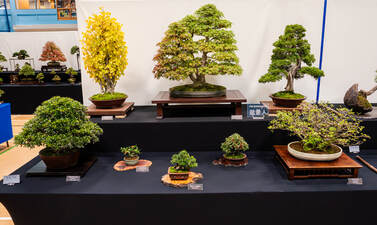
\includegraphics[angle=0,origin=c,width=1.0\textwidth]{2025_10/res/heathrow_34_the_bonsai_boys}
        \centerline{\emph{The Bonsai Boys}}
    \end{minipage}
\end{center}
\clearpage

\begin{center}
    \begin{minipage}[b]{.4\textwidth}
        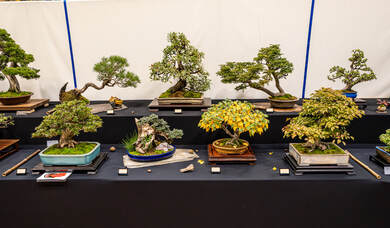
\includegraphics[angle=0,origin=c,width=1.0\textwidth]{2025_10/res/heathrow_35_twickenham_bonsai_society}
        \centerline{\emph{Twickenham Bonsai Society}}
    \end{minipage}\quad
    \begin{minipage}[b]{.4\textwidth}
        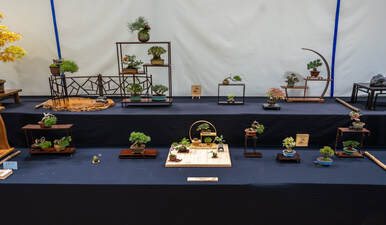
\includegraphics[angle=0,origin=c,width=1.0\textwidth]{2025_10/res/heathrow_36_uk_mini_bonsai_group}
        \centerline{\emph{UK Mini Bonsai Group}}
    \end{minipage}
    \medskip

    \begin{minipage}[b]{.4\textwidth}
        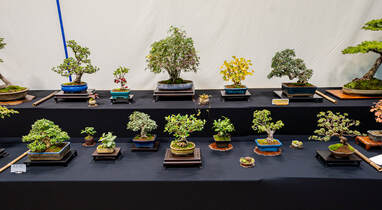
\includegraphics[angle=0,origin=c,width=1.0\textwidth]{2025_10/res/heathrow_37_warminster_bonsai_society}
        \centerline{\emph{Warminster Bonsai Society}}
    \end{minipage}\quad
    \begin{minipage}[b]{.4\textwidth}
        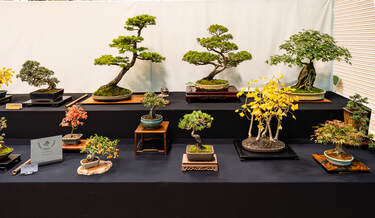
\includegraphics[angle=0,origin=c,width=1.0\textwidth]{2025_10/res/heathrow_38_wessex_bonsai_society}
        \centerline{\emph{Wessex Bonsai Society}}
    \end{minipage}
\end{center}
\medskip

\begin{center}
    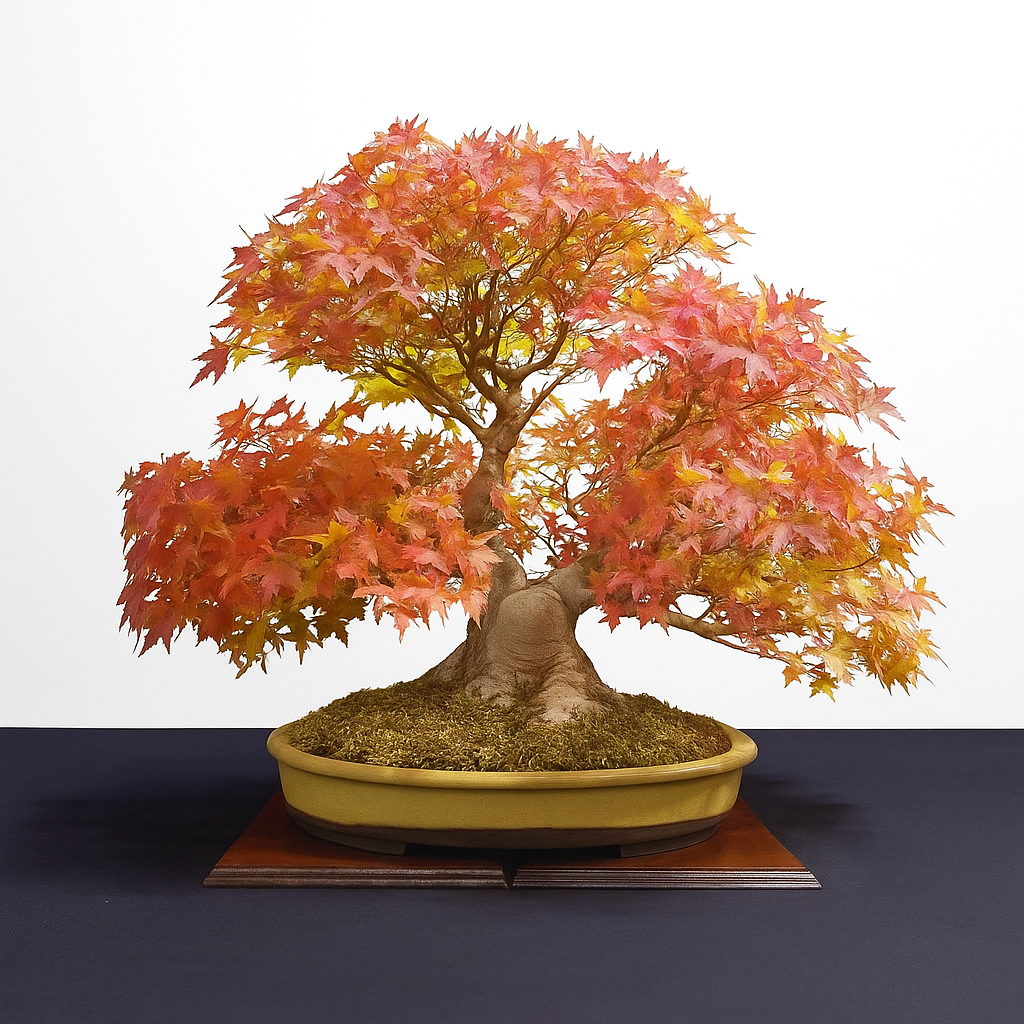
\includegraphics[width=0.75\columnwidth]{2025_10/res/heathrow_00_filler.png}
\end{center}

\begin{multicols}{2} 
\clearpage
